\begin{name}
	{\tenchude}{\tendethi}{LỚP TOÁN THẦY PHÁT}{\thoigian}
\end{name}
\setcounter{ex}{0}\setcounter{bt}{0}
\Opensolutionfile{ans}[ans/ans-2-TT-8-SGD-ThuaThienHue-23]
\begin{ex}%[Thi thử tốt nghiệp - SGD Thừa Thiên Huế - 23]%[Phạm Phương - EX6 - 23]%[2D2Y5-2]
	Xác định nghiệm của phương trình $5^{x-3}=25$.
	\choice
	{$x=3$}
	{$x=2$}
	{\True $x=5$}
	{$x=4$}
	\loigiai{
	Ta có $5^{x-3}=25 \Leftrightarrow 5^{x-3}=5^2 \Leftrightarrow x-3=2 \Leftrightarrow x=5$.
	}
\end{ex}
\begin{ex}%[Thi thử tốt nghiệp - SGD Thừa Thiên Huế - 23]%[Phạm Phương - EX6 - 23]%[2H2Y1-6]
	Tính thể tích của khối trụ tròn xoay có bán kính đáy $r$ và chiều cao $h$.
	\choice
	{$\dfrac{1}{3}\pi r^2 h$}
	{\True $\pi r^2 h$}
	{$2\pi r h$}
	{$\dfrac{4}{3} \pi r^2 h$}
	\loigiai{
	Thể tích khối trụ tính bởi công thức $V=\pi r^2 h$.
	}
\end{ex}
\begin{ex}%[Thi thử tốt nghiệp - SGD Thừa Thiên Huế - 23]%[Phạm Phương - EX6 - 23]%[2D3Y1-1]
	Khẳng định nào dưới đây đúng?
	\choice
	{$\displaystyle\int 4x^3 \mathrm{\,d}x=4x^4+C$}
	{$\displaystyle\int 4x^3 \mathrm{\,d}x=\dfrac{1}{4}x^4+C$}
	{$\displaystyle\int 4x^3 \mathrm{\,d}x=12x^2+C$}
	{\True $\displaystyle\int 4x^3 \mathrm{\,d}x=x^4+C$}
	\loigiai{
	Theo định nghĩa nguyên hàm ta có $\displaystyle\int 4x^3 \mathrm{\,d}x=4 \cdot \displaystyle\int x^3 \mathrm{\,d}x=4 \cdot \dfrac{x^4}{4}+C=x^4+C$.
	}
\end{ex}
\begin{ex}%[Thi thử tốt nghiệp - SGD Thừa Thiên Huế - 23]%[Phạm Phương - EX6 - 23]%[2D3Y2-1]
	Tính tích phân $I=\displaystyle\int\limits_0^1(2x-1) \mathrm{\,d}x$.
	\choice
	{$I=2$}
	{$I=3$}
	{\True $I=0$}
	{$I=1$}
	\loigiai{
	Ta có $I=\displaystyle\int\limits_0^1(2x-1) \mathrm{\,d}x=\left(x^2-x\right)\bigg|_0 ^1=\left(1^2-1\right)-\left(0^2-0\right)=0$.
}
\end{ex}
\begin{ex}%[Thi thử tốt nghiệp - SGD Thừa Thiên Huế - 23]%[Phạm Phương - EX6 - 23]%[2H3Y1-1]
	Trong KG $Oxyz$, cho điểm $A(1;-3;2)$ và $B(2;1;1)$. Hãy xác định toạ độ véc-tơ $\overrightarrow{AB}$.
	\choice
	{$\overrightarrow{AB}=(1;2;1)$}
	{$\overrightarrow{AB}=(1;-4;-1)$}
	{$\overrightarrow{AB}=(1;4;1)$}
	{\True $\overrightarrow{AB}=(1;4;-1)$}
	\loigiai{
	Ta có $\overrightarrow{AB}=(2-1;1-(-3);1-2)=(1;4;-1)$.
}
\end{ex}
\begin{ex}%[Thi thử tốt nghiệp - SGD Thừa Thiên Huế - 23]%[Phạm Phương - EX6 - 23]%[2D1Y1-2]
	Cho hàm số $y=f(x)$ xác định trên $\mathbb{R}$ và có bảng xét dấu đạo hàm như sau:
	\begin{center}
		
\begin{tikzpicture}
			\tkzTabInit[nocadre=false,lgt=1.2,espcl=2.5,deltacl=0.6]
			{$x$/0.6,$y'$/0.6}
			{$-\infty$,$-1$,$2$,$+\infty$}
			\tkzTabLine{,-,$0$,+,$0$,-,}
		\end{tikzpicture}
	\end{center}
	Khi đó hàm số $y=f(x)$ đồng biến trên khoảng nào?
	\choice
	{$(-\infty;-1)$}
	{\True $(-1;2)$}
	{$(-1;+\infty)$}
	{$(-\infty;2)$}
	\loigiai{
	Ta có $y'>0$ khi $x \in(-1;2)$. Do đó hàm số đồng biến trên khoảng $(-1;2)$.
	}
\end{ex}
\begin{ex}%[Thi thử tốt nghiệp - SGD Thừa Thiên Huế - 23]%[Phạm Phương - EX6 - 23]%[2D2Y1-2]
	Rút gọn biểu thức $Q=b^{\tfrac{4}{3}}:\sqrt[3]{b}$ với $b>0$ ta được
	\choice
	{$Q=b^4$}
	{$Q=b^2$}
	{\True $Q=b$}
	{$Q=b^3$}
	\loigiai{
		Ta có $Q=b^{\tfrac{4}{3}}: \sqrt[3]{b}=b^{\tfrac{4}{3}}: b^{\tfrac{1}{3}}=b^{\left(\tfrac{4}{3}-\tfrac{1}{3}\right)}=b^1=b$.
	}
\end{ex}
\begin{ex}%[Thi thử tốt nghiệp - SGD Thừa Thiên Huế - 23]%[Phạm Phương - EX6 - 23]%[2D3Y2-1]
	Biết $\displaystyle\int\limits_1^2 f(x) \mathrm{\,d}x=2$ và $\displaystyle\int\limits_1^2 g(x) \mathrm{\,d}x=3$. Tính giá trị của $\displaystyle\int\limits_1^2 \left[f(x)-2 g(x)\right] \mathrm{\,d}x$.
	\choice
	{\True $-4$}
	{$-1$}
	{$8$}
	{$1$}
	\loigiai{
	Ta có $\displaystyle\int\limits_1^2 \left[f(x)-2 g(x)\right] \mathrm{\,d}x=\displaystyle\int\limits_1^2 f(x) \mathrm{\,d}x-2 \cdot \displaystyle\int\limits_1^2 g(x) \mathrm{\,d}x=2-2\cdot 3=-4$.
	}
\end{ex}
\begin{ex}%[Thi thử tốt nghiệp - SGD Thừa Thiên Huế - 23]%[Phạm Phương - EX6 - 23]%[2H3Y1-1]
	Trong KG $Oxyz$, xác định toạ độ điểm $H$ là hình chiếu vuông góc của $A(1;-1;4)$ lên mặt phẳng $(Oyz)$.
	\choice
	{$H(1;0;0)$}
	{$H(1;0;4)$}
	{$H(0;-1;0)$}
	{\True $H(0;-1;4)$}
	\loigiai{
	Hình chiếu của $M(x_M;y_M;z_M)$ lên mặt phẳng $(Oyz)$ là $M'(0;y_M;z_M)$.\\
	Áp dụng ta có hình chiếu vuông góc của $A(1;-1;4)$ lên mặt phẳng $(Oyz)$ là $H(0;-1;4)$.
	}
\end{ex}
\begin{ex}%[Thi thử tốt nghiệp - SGD Thừa Thiên Huế - 23]%[Phạm Phương - EX6 - 23]%[2D1Y2-2]
	Cho hàm số $y=f(x)$ có bảng biến thiên như sau
	\begin{center}
		
\begin{tikzpicture}
			\tkzTabInit[nocadre=false,lgt=1.2,espcl=2.5,deltacl=0.6]
			{$x$/0.6,$f'(x)$/0.6,$f(x)$/2}
			{$-\infty$,$2$,$3$,$+\infty$}
			\tkzTabLine{,-,$0$,+,$0$,-,}
			\tkzTabVar{+/$+\infty$,-/$-1$,+/$2$,-/$-\infty$}
		\end{tikzpicture}
	\end{center}
	Xác định giá trị cực đại của hàm số $y=f(x)$.
	\choice
	{$x=2$}
	{$x=3$}
	{$y=-1$}
	{\True $y=2$}
	\loigiai{
	Hàm số đạt cực đại tại điểm $x=3$ và giá trị cực đại là $y_{\text{CĐ}}=2$.
}
\end{ex}
\begin{ex}%[Thi thử tốt nghiệp - SGD Thừa Thiên Huế - 23]%[Phạm Phương - EX6 - 23]%[2H1Y3-2]
	Cho khối chóp có diện tích đáy $B=8a^2$ và chiều cao $h=a$. Tính thể tích khối chóp đã cho.
	\choice
	{$\dfrac{4}{3}a^3$}
	{$4a^3$}
	{$8a^3$}
	{\True $\dfrac{8}{3}a^3$}
	\loigiai{
	Thể tích khối chóp là $V=\dfrac{1}{3} B \cdot h=\dfrac{1}{3} 8a^2 \cdot a=\dfrac{8a^3}{3}$.
	}
\end{ex}
\begin{ex}%[Thi thử tốt nghiệp - SGD Thừa Thiên Huế - 23]%[Phạm Phương - EX6 - 23]%[2H3Y1-1]
	Trong KG $Oxyz$, cho véc-tơ $\overrightarrow{OA}=-\vec{i}+\vec{j}+2\vec{k}$. Xác định toạ độ điểm $A$.
	\choice
	{\True $(-1;1;2)$}
	{$(-1;1;-2)$}
	{$(1;-1;2)$}
	{$(1;-1;-2)$}
	\loigiai{
	Ta có $\overrightarrow{OA}=-\vec{i}+\vec{j}+2 \vec{k} \Rightarrow \overrightarrow{OA}=(-1;1;2) \Rightarrow A(-1;1;2)$.
	}
\end{ex}
\begin{ex}%[Thi thử tốt nghiệp - SGD Thừa Thiên Huế - 23]%[Phạm Phương - EX6 - 23]%[2D2Y3-2]
	Với $a$ là số dương tuỳ ý, khi đó $\log_5 a^3$ bằng
	\choice
	{$3+\log_5 a$}
	{$\dfrac{1}{3}+\log_5 a$}
	{\True $3 \log_5 a$}
	{$\dfrac{1}{3} \log_5 a$}
	\loigiai{
	Theo công thức lôgarit của một luỹ thừa ta có $\log_5 a^3=3 \cdot \log_5 a$.
	}
\end{ex}
\begin{ex}%[Thi thử tốt nghiệp - SGD Thừa Thiên Huế - 23]%[Phạm Phương - EX6 - 23]%[2D1Y5-4]
	Xác định toạ độ giao điểm của đồ thị hàm số $y=\dfrac{3x-2}{x+1}$ với trục tung.
	\choice
	{$M(-2;0)$}
	{\True $M(0;-2)$}
	{$M\left(0;\dfrac{2}{3}\right)$}
	{$M\left(\dfrac{2}{3};0\right)$}
\loigiai{
	Giao điểm với trục tung $Oy$ (có phương trình $x=0$) nên ta có $x=0 \Rightarrow y=-2 \Rightarrow M(0;-2)$.
	}
\end{ex}
\begin{ex}%[Thi thử tốt nghiệp - SGD Thừa Thiên Huế - 23]%[Phạm Phương - EX6 - 23]%[2H3Y1-3]
	Xác định toạ độ tâm của mặt cầu $(S)\colon (x-1)^2+(y+2)^2+z^2=12$.
	\choice
	{$I(-2;2;12)$}
	{\True $I(1;-2;0)$}
	{$I(1;-2;-12)$}
	{$I(-1;2;0)$}
	\loigiai{
	Mặt cầu $(S)\colon (x-a)^2+(y-b)^2+(z-c)^2=R^2$ có tâm $I(a;b;c)$ và bán kính $R$.\\
	Áp dụng với $(S)\colon (x-1)^2+(y+2)^2+z^2=12$ ta có tâm $I(1;-2;0)$.
}
\end{ex}
\begin{ex}%[Thi thử tốt nghiệp - SGD Thừa Thiên Huế - 23]%[Phạm Phương - EX6 - 23]%[2D3Y1-1]
Cho $F(x)=\displaystyle\int\left(\mathrm{e}^x-1\right) \mathrm{\,d}x$. Trong các khẳng định sau, khẳng định nào đúng?
\choice
{$F(x)=\mathrm{e}^x+x+C$}
{\True $F(x)=\mathrm{e}^x-x+C$}
{$F(x)=\mathrm{e}^x+C$}
{$F(x)=-\mathrm{e}^x+x+C$}
\loigiai{
	Ta có $F(x)=\displaystyle\int\left(e^x-1\right) \mathrm{\,d}x=\displaystyle\int \mathrm{e}^x \mathrm{\,d}x-\displaystyle\int 1 \mathrm{\,d}x=\mathrm{e}^x-x+C$.
}
\end{ex}
\begin{ex}%[Thi thử tốt nghiệp - SGD Thừa Thiên Huế - 23]%[Phạm Phương - EX6 - 23]%[2D1Y5-1]
\immini{
Đồ thị hàm số nào dưới đây có dạng như đường cong trong hình bên?
\choice
{$y=x^2-3x+1$}
{\True $y=-x^4+2x^2+1$}
{$y=-x^3+3x+1$}
{$y=x^4-2x^2+1$}
}{
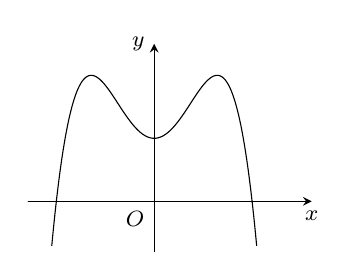
\begin{tikzpicture}[scale=0.8,>=stealth, font=\footnotesize, line join=round, line cap=round]
	\def\a{-1} \def\b{2} \def\c{1} % Hệ số
	\def\xmin{-2} \def\xmax{2.5}
	\def\ymin{-0.8} \def\ymax{2.5} 
	%\draw[color=gray!50,dashed] (\xmin,\ymin) grid (\xmax,\ymax);
	\draw[->] (\xmin,0)--(\xmax,0) node [below]{$x$};
	\draw[->] (0,\ymin)--(0,\ymax) node [left]{$y$};
	\node at (0,0) [below left]{$O$};
	\clip (\xmin+0.1,\ymin+0.1) rectangle (\xmax-0.5,\ymax-0.1);
	\draw[smooth,samples=300,domain=\xmin:\xmax] plot(\x,{\a*(\x)^4+\b*(\x)^2+\c});
\end{tikzpicture}
}
\loigiai{
	Dựa vào hình dạng đồ thị ta thấy đây là dạng đồ thị của hàm số bậc 4 trùng phương và có hệ số $a<0$ nên chỉ có hàm số $y=-x^4+2x^2+1$ thoả mãn.
}
\end{ex}
\begin{ex}%[Thi thử tốt nghiệp - SGD Thừa Thiên Huế - 23]%[Phạm Phương - EX6 - 23]%[2H3Y2-4]
Trong KG $Oxyz$, cho mặt phẳng $(P)\colon 2x-y-z-4=0$. Hãy xác định giao điểm của mặt phẳng $(P)$ và trục $Oz$.
\choice
{\True $M(0;0;-4)$}
{$M(0;0;4)$}
{$M(2;0;0)$}
{$M(-2;0;0)$}
\loigiai{
	$(P)$ giao với trục $Oz \Rightarrow x=y=0$. Thay $x=y=0$ vào phương trình của $(P)$ ta được $$2\cdot 0-0-z-4=0 \Leftrightarrow z=-4.$$
	Suy ra giao điểm của $(P)$ và trục $Oz$ là điểm $M(0;0;-4)$.
}
\end{ex}
\begin{ex}%[Thi thử tốt nghiệp - SGD Thừa Thiên Huế - 23]%[Phạm Phương - EX6 - 23]%[2D1Y4-1]
Xác định tiệm cận đứng của đồ thị hàm số $y=\dfrac{2x+1}{x-2}$.
\choice
{$y=2$}
{$y=-\dfrac{1}{2}$}
{\True $x=2$}
{$x=-\dfrac{1}{2}$}
\loigiai{
	Tiệm cận đứng của đồ thị hàm số $y=\dfrac{ax+b}{cx+d}$ là đường thẳng $x=-\dfrac{d}{c}$.\\
	Áp dụng với hàm số $y=\dfrac{2x+1}{x-2}$ ta có tiệm cận đứng là $x=-\dfrac{-2}{1} \Leftrightarrow x=2$.
}
\end{ex}
\begin{ex}%[Thi thử tốt nghiệp - SGD Thừa Thiên Huế - 23]%[Phạm Phương - EX6 - 23]%[2H3Y2-2]
	Trong KG $Oxyz$, hãy xác định toạ độ một véc-tơ pháp tuyến của mặt phẳng $(P)$ có phương trình $3x-y-z+2=0$.
	\choice
	{$\vec{n}=(-1;-1;2)$}
	{\True $\vec{n}=(3;-1;-1)$}
	{$\vec{n}=(3;1;1)$}
	{$\vec{n}=(3;-1;2)$}
	\loigiai{
	Mặt phẳng $(P)\colon Ax+By+Cz+D=0$ có một véc-tơ pháp tuyến là $\vec{n}=(A;B;C)$.\\
	Áp dụng với $(P)\colon 3x-y-z+2=0$ ta có $\vec{n}=(3;-1;-1)$.
	}
\end{ex}
\begin{ex}%[Thi thử tốt nghiệp - SGD Thừa Thiên Huế - 23]%[Phạm Phương - EX6 - 23]%[2H2Y1-2]
	Cho hình nón $(N)$ có bán kính đáy bằng $3$ và chiều cao bằng $4$. Xác định độ dài đường sinh của hình nón $(N)$.
	\choice
	{\True $5$}
	{$\sqrt{7}$}
	{$1$}
	{$12$}
	\loigiai{
	Độ dài đường sinh của hình nón là $$\ell=\sqrt{r^2+h^2}=\sqrt{3^2+4^2}=5.$$
	}
\end{ex}
\begin{ex}%[Thi thử tốt nghiệp - SGD Thừa Thiên Huế - 23]%[Phạm Phương - EX6 - 23]%[2D2Y4-2]
	Trên khoảng $(0;+\infty)$, xác định đạo hàm của hàm số $y=\log x$.
	\choice
	{\True $y'=\dfrac{1}{x \ln 10}$}
	{$y'=\dfrac{1}{10 \ln x}$}
	{$y'=\dfrac{1}{x}$}
	{$y'=\dfrac{\ln 10}{x}$}
	\loigiai{
		Ta có $\left(\log_a x\right)'=\dfrac{1}{x \ln a}$, áp dụng với $a=10$ ta có $y'=(\log x)'=(\log_{10} x)'=\dfrac{1}{x \ln 10}$.
	}
\end{ex}
\begin{ex}%[Thi thử tốt nghiệp - SGD Thừa Thiên Huế - 23]%[Phạm Phương - EX6 - 23]%[2D1B2-1]
	Xác định số điểm cực trị của hàm số $y=x^4-10x^2+1$.
	\choice
	{\True $3$}
	{$2$}
	{$0$}
	{$1$}
	\loigiai{
		Ta có $y'=4x^3-20x$.\\
		Khi đó $y'=0 \Leftrightarrow 4x^3-20x=0 \Leftrightarrow\hoac{&x=0\\&x=\sqrt{5}\\&x=-\sqrt{5}}$ (3 nghiệm đơn) nên hàm số có 3 điểm cực trị.
	}
\end{ex}
\begin{ex}%[Thi thử tốt nghiệp - SGD Thừa Thiên Huế - 23]%[Phạm Phương - EX6 - 23]%[2D1B3-1]
	Xác định giá trị nhỏ nhất của hàm số $y=x^3+x$ trên $[0;2]$.
	\choice
	{\True $0$}
	{$-2$}
	{$10$}
	{$2$}
	\loigiai{
		Ta có $y'=3x^2+1$, khi đó $y'=0 \Leftrightarrow 3x^2+1=0 \text{ (vô nghiệm)}$.\\
		Lại có $y(0)=0$ và $y(2)=10$ nên suy ra $\min\limits_{[0;2]} y=y(0)=0$.
	}
\end{ex}
\begin{ex}%[Thi thử tốt nghiệp - SGD Thừa Thiên Huế - 23]%[Phạm Phương - EX6 - 23]%[2H1B3-2]
	Cho khối lăng trụ có đáy là hình vuông cạnh bằng $a$ và chiều cao bằng $4a$. Tính thể tích của khối lăng trụ đã cho.
	\choice
	{$\dfrac{16}{3}a^3$}
	{$\dfrac{4}{3}a^3$}
	{$16a^3$}
	{\True $4a^3$}
	\loigiai{
		Diện tích đáy là $B=S_{ABCD}=a^2$.\\
		Thể tích khối lăng trụ là $V=B \cdot h=a^2 \cdot 4a=4a^3$.
	}
\end{ex}
\begin{ex}%[Thi thử tốt nghiệp - SGD Thừa Thiên Huế - 23]%[Phạm Phương - EX6 - 23]%[2D1B5-3]
	Cho hàm số $y=f(x)$ xác định, liên tục trên $\mathbb{R}$ và có bảng biến thiên như sau:
	\begin{center}
		\begin{tikzpicture}[scale=1, font=\footnotesize, line join=round, line cap=round, >=stealth]
			\tkzTabInit[nocadre=false,lgt=1.2,espcl=2,deltacl=0.6]
			{$x$ /0.6,$y'$ /0.6,$y$ /2}
			{$-\infty$,$-2$,$0$,$2$,$+\infty$}
			\tkzTabLine{,-,$0$,+,$0$,-,$0$,+,}
			\path
			(N12)--(N13)node[pos=0.1](A){$+\infty $}
			(N22)--(N23)node[pos=0.9](B){$-3$}
			(N32)--(N33)node[pos=0.4](C){$1$}
			(N42)--(N43)node[pos=0.9](D){$-3$}
			(N52)--(N53)node[pos=0.1](E){$+\infty $};
			\foreach \p/\q in{A/B,B/C,C/D,D/E} \draw[->] (\p)--(\q);
		\end{tikzpicture}
	\end{center}
	Xác định số nghiệm của phương trình $f(x)=1$.
	\choice
	{0}
	{2}
	{\True 3}
	{1}
	\loigiai{
		\begin{center}
			\begin{tikzpicture}[scale=1, font=\footnotesize, line join=round, line cap=round, >=stealth]
				\tkzTabInit[nocadre=true,lgt=1.2,espcl=2,deltacl=0.6]
				{$x$ /0.6,$y'$ /0.6,$y$ /2}
				{$-\infty$,$-2$,$0$,$2$,$+\infty$}
				\tkzTabLine{,-,$0$,+,$0$,-,$0$,+,}
				\path
				(N12)--(N13)node[pos=0.1](A){$+\infty $}
				(N22)--(N23)node[pos=0.9](B){$-3$}
				(N32)--(N33)node[pos=0.4](C){$1$}
				(N42)--(N43)node[pos=0.9](D){$-3$}
				(N52)--(N53)node[pos=0.1](E){$+\infty $};
				\foreach \p/\q in{A/B,B/C,C/D,D/E} \draw[->] (\p)--(\q);
				\draw[red,thick] ($(N12)!0.45!(N13)$)--($(N52)!0.45!(N53)$)node[below right]{$y=1$};
			\end{tikzpicture}
		\end{center}
		Kẻ đường thẳng $y=1$ (hình vẽ ở trên) ta thấy đồ thị hàm số $y=f(x)$ và đường thẳng $y=1$ có 3 điểm chung nên suy ra phương trình $f(x)=1$ có 3 nghiệm.
	}
\end{ex}
\begin{ex}%[Thi thử tốt nghiệp - SGD Thừa Thiên Huế - 23]%[Phạm Phương - EX6 - 23]%[2D1B1-3]
	Xác định tất cả các giá trị thực của tham số $m$ để hàm số $y=x^3-2x^2+mx-1$ đồng biến trên $\mathbb{R}$.
	\choice
	{$m \leq \dfrac{2}{3}$}
	{$m \geq 1$}
	{$m \leq 2$}
	{\True $m \geq \dfrac{4}{3}$}
	\loigiai{
	Ta có $y'=3x^2-4x+m$.\\
	Hàm số đồng biến trên $\mathbb{R} \Leftrightarrow y' \geq 0, \forall x \in \mathbb{R} \Leftrightarrow 3x^2-4x+m \geq 0, \forall x \in \mathbb{R}$. 
	$$\Leftrightarrow \heva{&a>0 \\& \Delta \leq 0} \Leftrightarrow \heva{&3>0 \\& (-4)^2-4\cdot 3\cdot m \leq 0} \Leftrightarrow  m \geq \dfrac{4}{3}.$$
}
\end{ex}
\begin{ex}%[Thi thử tốt nghiệp - SGD Thừa Thiên Huế - 23]%[Phạm Phương - EX6 - 23]%[2H3B2-4]
	Trong KG $Oxyz$, cho mặt phẳng $(P)\colon 2x-z+1=0$. Điểm nào trong các điểm sau thuộc mặt phẳng $(P)$?
	\choice
	{\True $M(1;7;3)$}
	{$M(0;-3;0)$}
	{$M(0;3;2)$}
	{$M(1;3;0)$}
	\loigiai{
\begin{itemize}
	\item Với $M(1;7;3)$ ta có $2x-z+1=2\cdot 1-3+1=-1 = 0$ nên $M(1;7;3) \in (P)$.
	\item Với $M(0;-3;0)$ ta có $2x-z+1=2\cdot 0-0+1=1 \neq 0$ nên $M(0;-3;0) \notin (P)$.
	\item Với $M(0;3;2)$ ta có $2x-z+1=2\cdot 0-2+1=-1 \neq 0$ nên $M(0;3;2) \notin (P)$.
	\item Với $M(1;3;0)$ ta có $2x-z+1=2\cdot 1-0+1=3 \neq 0$ nên $M(1;3;0) \notin (P)$.
\end{itemize}	
}
\end{ex}
\begin{ex}%[Thi thử tốt nghiệp - SGD Thừa Thiên Huế - 23]%[Phạm Phương - EX6 - 23]%[2D2B1-2]
	Tính giá trị của biểu thức $2^{2x+1}$ biết rằng $2^x=5$.
	\choice
	{$10$}
	{$11$}
	{\True $50$}
	{$25$}
	\loigiai{
	Ta có $2^{2x+1}=2^{2x} \cdot 2^1=\left(2^x\right)^2 \cdot 2=5^2 \cdot 2=50$.
}
\end{ex}
\begin{ex}%[Thi thử tốt nghiệp - SGD Thừa Thiên Huế - 23]%[Phạm Phương - EX6 - 23]%[2D2B2-1]
	Tìm tập xác định $\mathscr{D}$ của hàm số $y=(x-1)^{-3}$.
	\choice
	{$\mathscr{D}=(1;+\infty)$}
	{\True $\mathscr{D}=\mathbb{R} \setminus \{1\}$}
	{$\mathscr{D}=\mathbb{R}$}
	{$\mathscr{D}=(-\infty;1)$}
	\loigiai{
	Vì số mũ $\alpha=-3$ là số nguyên âm nên điều kiện xác định là
	$$x-1 \neq 0 \Leftrightarrow x \neq 1.$$
	Suy ra tập xác định là $\mathscr{D}=\mathbb{R}\setminus \{1\}$.
	}
\end{ex}
\begin{ex}%[Thi thử tốt nghiệp - SGD Thừa Thiên Huế - 23]%[Phạm Phương - EX6 - 23]%[2D3B3-1]
	Xác định công thức tính thể tích vật thể tròn xoay sinh ra bởi hình phẳng giới hạn bởi các đường $y=\sqrt{2x+1}$, $y=0$, $x=0$, $x=4$ khi quay quanh trục $Ox$.
	\choice
	{$V=\pi \displaystyle\int\limits_0^4 \sqrt{2x+1} \mathrm{\,d}x$}
	{$V=\displaystyle\int\limits_0^4(2x+1) \mathrm{\,d}x$}
	{\True $V=\pi \displaystyle\int\limits_0^4(2x+1) \mathrm{\,d}x$}
	{$V=\displaystyle\int\limits_0^4 \sqrt{2x+1} \mathrm{\,d}x$}
	\loigiai{
	Thể tích vật thể tròn xoay sinh ra bởi hình phẳng giới hạn bởi các đường $y=f(x)$, $y=0$, $x=a$, $x=b$ $(b>a)$ khi quay quanh trục $Ox$ là
	$$V=\pi \displaystyle\int\limits_a^b \left[f(x)\right]^2 \mathrm{\,d}x.$$
	Từ yêu cầu của bài toán ta có
	$$V=\pi \displaystyle\int\limits_0^4 \left(\sqrt{2x+1}\right)^2 \mathrm{\,d}x=\pi \displaystyle\int\limits_0^4 \left(2x+1\right) \mathrm{\,d}x.$$
	}
\end{ex}
\begin{ex}%[Thi thử tốt nghiệp - SGD Thừa Thiên Huế - 23]%[Phạm Phương - EX6 - 23]%[2H1B3-1]
	Cho hình lập phương có thể tích bằng $2a^3\sqrt{2}$. Tính diện tích một mặt của hình lập phương.
	\choice
	{\True $2a^2$}
	{$a^2 \sqrt{2}$}
	{$a^2$}
	{$2a^2 \sqrt{2}$}
	\loigiai{
		Gọi $x$ là độ dài cạnh của hình lập phương.	Khi đó thể tích của khối lập phương là
		$$x^3=2a^3 \sqrt{2}=\left(a\sqrt{2}\right)^3 \Rightarrow x=a \sqrt{2}.$$
		Suy ra diện tích một mặt của khối lập phương là
		$$S=x^2=\left(a \sqrt{2}\right)^2=2a^2.$$
	}
\end{ex}
\begin{ex}%[Thi thử tốt nghiệp - SGD Thừa Thiên Huế - 23]%[Phạm Phương - EX6 - 23]%[2D2B6-2]
	Xác định tập nghiệm của bất phương trình $\log_3(x-1) \geq 1$.
	\choice
	{\True $[4;+\infty)$}
	{$(4;+\infty)$}
	{$(1;+\infty)$}
	{$[1;+\infty)$}
	\loigiai{
	Điều kiện $x-1>0 \Leftrightarrow x>1$.\\
	Ta có $\log_3(x-1) \geq 1 \Leftrightarrow x-1 \geq 3^1 \Leftrightarrow x \geq 4$.\\
	Kết hợp điều kiện ta được tập nghiệm củABất phương trình đã cho là $S=[4;+\infty)$.
	}
\end{ex}
\begin{ex}%[Thi thử tốt nghiệp - SGD Thừa Thiên Huế - 23]%[Phạm Phương - EX6 - 23]%[2D3B2-2]
	Cho $I=\displaystyle\int\limits_1^2 x\sqrt{x^2+1} \mathrm{\,d}x$. Đặt $t=x^2+1$, khi đó $I=\displaystyle\int\limits_1^2 x\sqrt{x^2+1} \mathrm{\,d}x$ trở thành biểu thức nào sau đây?
	\choice
	{$I=\displaystyle\int\limits_1^2 t \sqrt{t} \mathrm{\,d}t$}
	{$I=\displaystyle\int\limits_2^5 t \sqrt{t} \mathrm{\,d}t$}
	{\True $I=\dfrac{1}{2} \displaystyle\int\limits_2^5 \sqrt{t} \mathrm{\,d}t$}
	{$I=\dfrac{1}{2} \displaystyle\int\limits_1^2 \sqrt{t} \mathrm{\,d}t$}
	\loigiai{
		Đặt $t=x^2+1 \Rightarrow \mathrm{\,d}t=2x \mathrm{\,d}x \Rightarrow x \mathrm{\,d}x=\dfrac{\mathrm{\,d}t}{2}$.\\
		Đổi cận: $\heva{&x=1 \Rightarrow t=1^2+1=2\\&x=2 \Rightarrow t=2^2+1=5.}$\\
		Lúc đó ta có $I=\displaystyle\int\limits_1^2 x \sqrt{x^2+1} \mathrm{\,d}x=\displaystyle\int\limits_1^2 \sqrt{x^2+1} \cdot x \mathrm{\,d}x=\displaystyle\int\limits_2^5 \sqrt{t} \cdot \dfrac{\mathrm{\,d}t}{2}=\dfrac{1}{2} \displaystyle\int\limits_2^5 \sqrt{t}\mathrm{\,d}t$.}
\end{ex}
\begin{ex}%[Thi thử tốt nghiệp - SGD Thừa Thiên Huế - 23]%[Phạm Phương - EX6 - 23]%[2H3B2-3]
	Trong KG $Oxyz$, cho điểm $A(-2;0;6)$. Hãy xác định phương trình mặt phẳng trung trực của đoạn thẳng $OA$.
	\choice
	{$x-3y+1=0$}
	{$x-3y-1=0$}
	{$x-3z+20=0$}
	{\True $x-3z+10=0$}
	\loigiai{
	Gọi $M$ là trung điểm của đoạn thẳng $OA$. Khi đó ta có $M(-1;0;3)$.\\
	Mặt phẳng trung trực của đoạn thẳng $OA$ đi qua điểm $M(-1;0;3)$ và vuông góc với $OA$ nên nhận $\overrightarrow{OA}=(-2;0;6)=-2(1;0;-3)$ làm véc-tơ pháp tuyến, do đó có phương trình là $$1(x+1)+0(y-0)-3(z-3)=0 \Leftrightarrow x-3z+10=0.$$
	}
\end{ex}
\begin{ex}%[Thi thử tốt nghiệp - SGD Thừa Thiên Huế - 23]%[Phạm Phương - EX6 - 23]%[2H3B2-7]
	Trong KG $Oxyz$, cho mặt phẳng $(\alpha)\colon x-y+2z-7=0$. Hãy xác định mặt phẳng vuông góc với mặt phẳng $(\alpha)$ trong các mặt phẳng có phương trình sau
	\choice
	{$x+y-2z+7=0$}
	{$x-y-2z+7=0$}
	{\True $x+y+7=0$}
	{$x-y+7=0$}
	\loigiai{
		Mặt phẳng $(\alpha)$ có một véc-tơ pháp tuyến là $\overrightarrow{n}_{\alpha}=(1;-1;2)$.\\
		Xét mặt phẳng $x+y+7=0$ có véc-tơ pháp tuyến $\overrightarrow{n}_P=(1;1;0) \Rightarrow \overrightarrow{n}_P \cdot \overrightarrow{n}_{\alpha}=1\cdot 1+1\cdot (-1)+0\cdot 2=0$ nên suy ra $(P) \perp(\alpha)$. 
	}
\end{ex}
\begin{ex}%[Thi thử tốt nghiệp - SGD Thừa Thiên Huế - 23]%[Phạm Phương - EX6 - 23]%[2H1K3-4]
	Cho hình chóp $S.ABC$ có đáy là tam giác vuông cân tại $B$ và $AC=2a$. Cạnh bên $SA=4a$ và hợp với đáy một góc bằng $60^{\circ}$. Tính thể tích khối chóp $S.ABC$.
	\choice
	{$V_{S.ABC}=\dfrac{a^3 \sqrt{6}}{3}$}
	{$V_{S.ABC}=\dfrac{2a^3}{3}$}
	{$V_{S.ABC}=\dfrac{2a^3 \sqrt{6}}{3}$}
	{\True $V_{S.ABC}=\dfrac{2a^3 \sqrt{3}}{3}$}
	\loigiai{
		\immini{
			Xét $\triangle ABC$ vuông cân tại $B$ ta có
			$$\sin 45^{\circ}=\dfrac{AB}{AC} \Rightarrow AB=AC \cdot \sin 45^{\circ}=2a \cdot \dfrac{\sqrt{2}}{2}=a \sqrt{2}.$$
			Diện tích đáy là $S_{\triangle ABC}=\dfrac{1}{2} \cdot BA \cdot BC=\dfrac{1}{2} \cdot a\sqrt{2} \cdot a\sqrt{2}=a^2$.\\
			Gọi $H$ là hình chiếu vuông góc của $S$ lên $(ABC)$.
			Lúc đó ta có $$\left(SA,(ABC)\right)=(SA,HA)=\widehat{SAH}=60^{\circ}.$$
		}{
			\begin{tikzpicture}[scale=1,>=stealth, font=\footnotesize, line join=round, line cap=round]
				\coordinate (A) at (0,0);
				\coordinate (B) at (2.5,-1.2);
				\coordinate (C) at (3.5,0);
				\coordinate (H) at (1.8,-0.4);
				\coordinate (S) at ($(H)+(0,2.6)$);
				\draw (S)--(A)--(B)--(C)--(S)--(B);
				\draw[dashed] (A)--(C) (S)--(H)--(A);
				\foreach \p/\r in {S/90,A/180,B/-90,C/-45,H/0}
				\fill (\p) circle (1pt) node[shift={(\r:3mm)}]{$\p$};
				\foreach \s/\t/\k in {A/B/C, S/H/A} \draw    pic[ draw=black, angle eccentricity=0.75, angle radius=0.15cm]{right angle=\s--\t--\k};
				\draw (A)pic["$60^{\circ}$",draw=black,angle eccentricity=1.65,angle radius=0.4cm]{angle=H--A--S};
			\end{tikzpicture}
		}	
		\noindent Xét tam giác $SHA$ vuông tại $H$ ta có $\sin 60^{\circ}=\dfrac{SH}{SA} \Rightarrow SH=SA \cdot \sin 60^{\circ}=4a \cdot \dfrac{\sqrt{3}}{2}=2a \sqrt{3}$.\\
		Thể tích khối chóp $S.ABC$ là $V_{S.ABC}=\dfrac{1}{3} \cdot S_{\triangle ABC} \cdot SH=\dfrac{1}{3} \cdot a^2 \cdot 2a\sqrt{3}=\dfrac{2a^3\sqrt{3}}{3}$.
	}
\end{ex}
\begin{ex}%[Thi thử tốt nghiệp - SGD Thừa Thiên Huế - 23]%[Phạm Phương - EX6 - 23]%[2D1K5-3]
	Cho hàm số $f(x)=-x^4+2x^2+5$. Xác định tất cả các giá trị thực của tham số $m$ để phương trình $f(x)=m$ có bốn nghiệm phân biệt.
	\choice
	{$m \in(1;2)$}
	{\True $m \in(5;6)$}
	{$m \in(4;5)$}
	{$m \in(3;4)$}
	\loigiai{
		Ta có $f'(x)=-4x^3+4x$.
		Khi đó $f'(x)=0 \Leftrightarrow-4x^3+4x=0 \Leftrightarrow\hoac{&x=0\\&x=1\\&x=-1.}$\\
		Bảng biến thiên
		\begin{center}
			
\begin{tikzpicture}
				\tkzTabInit[nocadre=false,lgt=1.2,espcl=2.5,deltacl=0.6]
				{$x$/0.6,$y'$/0.6,$y$/2}
				{$-\infty$,$-1$,$0$,$1$,$+\infty$}
				\tkzTabLine{,+,$0$,-,$0$,+,$0$,-,}
				\tkzTabVar{-/$-\infty$,+/$6$,-/$5$,+/$6$,-/$-\infty$}
			\end{tikzpicture}
		\end{center}
		Dựa vào bảng biến thiên suy ra phương trình $f(x)=m$ có bốn nghiệm phân biệt $\Leftrightarrow 5<m<6$.
	}
\end{ex}
\begin{ex}%[Thi thử tốt nghiệp - SGD Thừa Thiên Huế - 23]%[Phạm Phương - EX6 - 23]%[2D1K4-2]
	Có bao nhiêu cặp số $(a;d)$ với $a$, $d$ là các số nguyên sao cho đồ thị hàm số $y=\dfrac{ax+24}{x+d}$ cắt trục hoành và trục tung tại hai điểm phân biệt $A$, $B$ đồng thời đường thẳng đi qua hai điểm $A$, $B$ đi qua giao hai đường tiệm cận của đồ thị hàm số $y=\dfrac{ax+24}{x+d}$.
	\choice
	{$32$}
	{$6$}
	{\True $12$}
	{$24$}
	\loigiai{
		Đồ thị hàm số có tiệm cận $\Leftrightarrow ad-bc \neq 0 \Leftrightarrow ad-24 \neq 0 \Leftrightarrow ad \neq 24$.\\
		Lúc đó tiệm cận đứng là $x+d=0 \Leftrightarrow x=-d$ và tiệm cận ngang là $y=\dfrac{a}{1} \Leftrightarrow y=a$.\\
		Suy ra giao điểm của 2 đường tiệm cận là $I(-d;a)$.\\
		Giao điểm của đồ thị hàm số và trục hoành  là $A\left(-\dfrac{24}{a};0\right)$, với $a \neq 0$.\\
		Giao điểm của đồ thị hàm số và trục tung là $B\left(0;\dfrac{24}{d}\right)$, với $d \neq 0$.\\
		PTĐT đi qua 2 điểm $A$, $B$ là $\dfrac{x}{-\tfrac{24}{a}}+\dfrac{y}{\tfrac{24}{d}}=1 \Leftrightarrow-\dfrac{ax}{24}+\dfrac{dy}{24}=1 \Leftrightarrow-ax+dy-24=0$.\\
		Đường thẳng $AB$ đi qua điểm $I(-d;a) \Leftrightarrow-a(-d)+d \cdot a-24=0 \Leftrightarrow ad=12$. (thoả mãn)\\
		Do $(a;d)$ nguyên nên suy ra số cặp $(a;d)$ thoả mãn $ad=12$ bằng số ước của 12 (tương ứng mỗi $a$ là ước của 12 ta tìm được $d=\dfrac{12}{a}$).
		Mặt khác, số 12 có 12 ước nguyên là $\pm 1;\pm 2;\pm 3;\pm 4;\pm 6;\pm 12$ nên suy ra có 12 cặp số nguyên $(a;d)$ thoả mãn đề bài.
	}
\end{ex}
\begin{ex}%[Thi thử tốt nghiệp - SGD Thừa Thiên Huế - 23]%[Phạm Phương - EX6 - 23]%[2H1K3-4]
	Cho hình chóp $S.ABCD$ có đáy $ABCD$ là hình vuông cạnh $2a$ và cạnh bên $SA$ vuông góc với đáy. Biết rằng khoảng cách từ $D$ đến mặt phẳng $(SBC)$ bằng $a\sqrt{3}$, tính thể tích khối chóp $S.ABCD$.
	\choice
	{\True $V=\dfrac{8a^3 \sqrt{3}}{3}$}
	{$V=\dfrac{4a^3 \sqrt{3}}{9}$}
	{$V=\dfrac{4a^3 \sqrt{3}}{3}$}
	{$V=\dfrac{8a^3 \sqrt{3}}{9}$}
	\loigiai{
		\immini{
		Diện tích đáy $S_{ABCD}=(2a)^2=4a^2$.\\
	Gọi $H$ là hình chiếu của $A$ lên $SB$, ta có
$$\heva{&AH \perp SB \\& AH \perp BC(\text { do} BC \perp(SAB)) }\Rightarrow AH \perp(SBC).$$
	Ta có $AD \parallel BC$ nên  $AD \parallel (SBC)$. Do đó
\begin{eqnarray*}
	\mathrm{d}\left(D,(SBC)\right)=\mathrm{d}\left(A,(SBC)\right)=AH=a\sqrt{3}. 
\end{eqnarray*}
}{
\begin{tikzpicture}[scale=0.8,>=stealth, font=\footnotesize, line join=round, line cap=round]
	\coordinate (A) at (0,0);
	\coordinate (B) at (-1.3,-1.2);
	\coordinate (D) at (3.5,0);
	\coordinate (C) at ($(B)+(D)-(A)$);
	\coordinate (S) at ($(A)+(0,2.6)$);
	\coordinate (H) at ($(S)!0.35!(B)$);
	\draw (S)--(B)--(C)--(D)--cycle;
	\draw (S)--(B) (S)--(C);
	\draw[dashed] (A)--(B) (A)--(D) (S)--(A) (A)--(H);
	\foreach \p/\r in {S/90,A/-45,B/-90,C/-45,D/0,H/150}
	\fill (\p) circle (1pt) node[shift={(\r:3mm)}]{$\p$};
	\foreach \s/\t/\k in {A/H/B}
	\draw pic[draw=black,angle eccentricity=0.75,angle radius=0.2cm]{right angle=\s--\t--\k};
\end{tikzpicture}
}
\noindent Xét tam giác $SAB$ vuông tại $A$ và $AH$ là đường cao, ta có
$$\dfrac{1}{AH^2}=\dfrac{1}{AB^2}+\dfrac{1}{AS^2} \Rightarrow \dfrac{1}{(a \sqrt{3})^2}=\dfrac{1}{(2a)^2}+\dfrac{1}{AS^2} \Rightarrow AS=2a \sqrt{3}.$$
Vậy thể tích khối chóp $S.ABCD$ là $V_{S.ABCD}=\dfrac{1}{3} \cdot S_{ABCD} \cdot SA=\dfrac{1}{3} \cdot 4a^2 \cdot 2a \sqrt{3}=\dfrac{8a^3\sqrt{3}}{3}$.
}
\end{ex}
\begin{ex}%[Thi thử tốt nghiệp - SGD Thừa Thiên Huế - 23]%[Phạm Phương - EX6 - 23]%[2D1K3-3]
Có bao nhiêu giá trị $m \in \mathbb{Z}$ để hàm số $g(x)=\left|\dfrac{2x-m}{x+2}\right|$ đạt giá trị nhỏ nhất trên đoạn $[-1;5]$ tại điểm $x=a \in(-1;5)$.
\choice
{$7$}
{\True $12$}
{$11$}
{$5$}
\loigiai{
	Xét hàm số $f(x)=\dfrac{2x-m}{x+2}$ có tập xác định là $D=\mathbb{R} \setminus \{-2\}$, nên hàm số xác định trên $[-1;5]$. \\
	Ta có $f'(x)=\dfrac{a d-b c}{(x+2)^2}=\dfrac{4+m}{(x+2)^2}$.
	\begin{itemize}
		\item [\bf TH1.] Với $m+4=0 \Leftrightarrow m=-4$ ta có $f(x)=\dfrac{2x+4}{x+2}=2$, với mọi $x \in \mathbb{R} \setminus \{-2\}$.\\
		Khi đó $g(x)=|f(x)|=2$, với mọi $x \in \mathbb{R} \backslash\{-2\}$ nên suy ra hàm số $g(x)$ đạt giá trị nhỏ nhất bằng 2 trên $[-1;5]$ tại mọi điểm $x=a \in(-1;5)$, do đó $m=-4$ thoả mãn yêu cầu bài toán.
		\item [\bf TH2.] Với $m+4 \neq 0 \Leftrightarrow m \neq-4$ ta có $f(x)$ là hàm đơn điệu (hoặc là tăng hoặc là giảm trên các khoảng xác định). Do đó hàm số $g(x)=\left|f(x)\right|$ đạt giá trị nhỏ nhất trên đoạn $[-1;5]$ tại điểm $x=a \in(-1;5)$ khi và chỉ khi phương trình $f(x)=0$ có nghiệm $a \in(-1;5)$.\\
		Lại có $f(x)=0 \Leftrightarrow 2x-m=0 \Leftrightarrow x=\dfrac{m}{2}$ nên theo đề ta có $-1<\dfrac{m}{2}<5 \Leftrightarrow-2<m<10$.\\
		Do $m$ nguyên nên $m \in\{-1;0;1;\ldots;8;9\}$.
	\end{itemize}
	Do đó có tất cả $12$ giá trị $m$ thoả mãn đề bài.
}
\end{ex}
\begin{ex}%[Thi thử tốt nghiệp - SGD Thừa Thiên Huế - 23]%[Phạm Phương - EX6 - 23]%[2D1K2-6]
Có bao nhiêu số nguyên $m$ để hàm số $y=f\left(x^2\right)+f\left(m-x^2\right)$ có đúng một điểm cực trị thuộc khoảng $(0;5)$, với $f(x)=x^6-x^4+x^2+x$?
\choice
{\True $49$}
{$7$}
{$12$}
{$13$}
\loigiai{
	Xét $y=h(x)=f\left(x^2\right)+f\left(m-x^2\right)$, ta có $y'=2x \cdot f'\left(x^2\right)-2x \cdot f'\left(m-x^2\right)=2x\left[f'\left(x^2\right)-f'\left(m-x^2\right)\right]$.
		Lúc đó 
		\begin{eqnarray*}
		y'=0 \Leftrightarrow \hoac{& 2x=0 \\ & f'\left(x^2\right)-f'\left(m-x^2\right)=0} \Leftrightarrow \hoac{&x=0 \\& f'\left(x^2\right)=f'\left(m-x^2\right). \quad (1)}
		\end{eqnarray*}
		Mặt khác, xét $f(x)=x^6-x^4+x^2+x$, ta có $f'(x)=6x^5-4x^3+2x+1 \Rightarrow f^{\prime \prime}(x)=30x^4-12 x^2+2$.\\
		Ta có $f ''(x)=0$ vô nghiệm và $a=30>0$ nên $f ''(x)>0$ với mọi $x \in \mathbb{R}$. Suy ra $f'(x)$ là hàm số đồng biến trên $\mathbb{R}$.\\
	Do đó $(1) \Leftrightarrow x^2=m-x^2 \Leftrightarrow 2x^2=m \Leftrightarrow x^2=\dfrac{m}{2}$. \quad (2)
	\begin{itemize}
		\item[\bf TH1.] Nếu $m<0$ thì phương trình $(2)$ vô nghiệm nên $h'(x)=0$ có nghiệm duy nhất là $x=0$ nên $x=0$ là cực trị duy nhất của hàm số $y=h(x)$. Do $x=0 \not\in(0;5)$ nên trường hợp này không thoả mãn.
		\item [\bf TH2.]  Nếu $m=0$ thì phương trình $(2)$ có nghiệm kép $x=0$ nên $h'(x)=0$ có nghiệm  $x=0$ là nghiệm bội 3 nên $x=0$ là cực trị duy nhất của hàm số $y=h(x)$. Do $x=0 \not\in(0;5)$ nên trường hợp này không thoả mãn.
		\item [\bf TH3.] Nếu $m>0$ thì phương trình $(3)$ có hai nghiệm phân biệt là $x_1=-\sqrt{\dfrac{m}{2}}<0$ và $x_2=\sqrt{\dfrac{m}{2}}>0$. Khi đó phương trình $h'(x)=0$ có 3 nghiệm phân biệt là $x=0$, $x=x_1$ và $x=x_2$ nên hàm số $h(x)$ có 3 điểm cực trị là $x=0$, $x=x_1$ và $x=x_2$.\\
		Do đó, hàm số có cực trị thuộc $(0;5) \Leftrightarrow x_2 \in(0;5) \Leftrightarrow 0<\sqrt{\dfrac{m}{2}}<5 \Leftrightarrow 0<\dfrac{m}{2}<25 \Leftrightarrow 0<m<50$.
		Lại có $m$ nguyên nên $m \in\{1;2;3;\ldots;49\}$.
	\end{itemize} 
	  Vậy có 49 giá trị $m$ thoả mãn đề bài.
	}
\end{ex}
\begin{ex}%[Thi thử tốt nghiệp - SGD Thừa Thiên Huế - 23]%[Phạm Phương - EX6 - 23]%[2D3K2-4]
	Cho hàm số $y=f(x)$ liên tục trên $\mathbb{R}$ và thoả mãn $f(x)+x=\displaystyle\int\limits_0^2[f(x)-x] \mathrm{\,d}x$, với mọi $x \in \mathbb{R}$. Xác định giá trị $m$ để $\displaystyle\int\limits_0^2 \left[mx+f(x)\right] \mathrm{\,d}x=0$.
	\choice
	{$m=0$}
	{$m=-2$}
	{$m=-1$}
	{\True $m=-3$}
	\loigiai{
		Đặt $k=\displaystyle\int\limits_0^2 f(x) \mathrm{\,d}x$. Ta có
		\begin{eqnarray*}
		& & 	f(x)+x=\displaystyle\int\limits_0^2[f(x)-x] \mathrm{\,d}x=\displaystyle\int\limits_0^2 f(x) \mathrm{\,d}x-\displaystyle\int\limits_0^2 x \mathrm{\,d}x=k-2 \quad (1)\\
		& \Leftrightarrow & f(x)=-x+k-2.
		\end{eqnarray*}
		Mặt khác, lấy tích phân cận từ $0$ tới $2$ hai vế của (1) ta được
		\begin{eqnarray*}
		& &\displaystyle\int\limits_0^2 f(x) \mathrm{\,d}x+\displaystyle\int\limits_0^2 x \mathrm{\,d}x=\displaystyle\int\limits_0^2(k-2) \mathrm{\,d}x \\
		& \Leftrightarrow & k+2=2(k-2) \Leftrightarrow k=6.
		\end{eqnarray*}
		Suy ra $f(x)=-x+4$, thử lại thấy thoả mãn $f(x)+x=\displaystyle\int\limits_0^2[f(x)-x] \mathrm{\,d}x$, với mọi $x \in \mathbb{R}$.\\
		Theo đề $\displaystyle\int\limits_0^2[mx+f(x)] \mathrm{\,d}x=0 \Leftrightarrow m \displaystyle\int\limits_0^2 x \mathrm{\,d}x + \displaystyle\int\limits_0^2 f(x) \mathrm{\,d}x =0 \Leftrightarrow 2m+6=0 \Leftrightarrow m=-3$.
}
\end{ex}
\begin{ex}%[Thi thử tốt nghiệp - SGD Thừa Thiên Huế - 23]%[Phạm Phương - EX6 - 23]%[2D3K2-4]
	Cho hàm số $y=f(x)$ có bảng biến thiên như sau
	\begin{center}
		
\begin{tikzpicture}
			\tkzTabInit[nocadre=false,lgt=1.2,espcl=2.5,deltacl=0.6]
			{$x$ /0.6, $f'(x)$ /0.6, $f(x)$ /2}
			{$-\infty$,$0$,$3$,$+\infty$}
			\tkzTabLine{,-,$0$,+,$0$,-,}
			\tkzTabVar{+/$+\infty$,-/$-1$,+/$5$,-/$-\infty$}
		\end{tikzpicture}
	\end{center}
	Xác định tất cả các giá trị thực của tham số $m$ để hàm số $F(x)=\displaystyle\int\left[f(x)+m\right] \mathrm{\,d} x$ nghịch biến trên khoảng $(0;3)$.
	\choice
	{$-5 \leq m \leq 1$}
	{\True $m \leq -5$}
	{$-1 \leq m \leq 5$}
	{$m \geq-1$}
	\loigiai{
		Ta có $F(x)=\displaystyle\int\left[f(x)+m\right] \mathrm{\,d}x \Rightarrow F'(x)=f(x)+m$.
		Hàm số $F(x)$ nghịch biến trên $(0;3)$ 
		\begin{eqnarray*}
			& \Leftrightarrow & F'(x) \leq 0, \forall x \in(0;3) \Leftrightarrow f(x)+m \leq 0, \forall x \in(0;3) \Leftrightarrow \max\limits_{x \in[0;3]}(f(x)+m) \leq 0. \quad (*)
		\end{eqnarray*}
Ta có bảng biến thiên của $f(x)+m$ trên $[0;3]$ như sau
\begin{center}
	
\begin{tikzpicture}
		\tkzTabInit[nocadre=false,lgt=1.8,espcl=4.5,deltacl=0.8]
		{$x$/0.6,$f'(x)$/0.6,$f(x)+m$/2}
		{$0$,$3$}
		\tkzTabLine{$0$,+,$0$}
		\tkzTabVar{-/$-1+m$,+/$5+m$}
	\end{tikzpicture}
\end{center}
Do đó $(*) \Leftrightarrow m+5 \leq 0 \Leftrightarrow m \leq -5.$	
}
\end{ex}
\begin{ex}%[Thi thử tốt nghiệp - SGD Thừa Thiên Huế - 23]%[Phạm Phương - EX6 - 23]%[2H2K1-3]
	Cho khối nón đỉnh $S$ có thể tích bằng $20 \pi$. Gọi $A$, $B$, $C$ là các điểm thuộc đường tròn đáy sao cho tam giác $ABC$ vuông cân. Tính thể tích khối chóp $S.ABC$.
	\choice
	{$V_{S.ABC}=\dfrac{20 \pi}{3}$}
	{$V_{S.ABC}=\pi$}
	{$V_{S.ABC}=\dfrac{20}{3}$}
	{\True $V_{S.ABC}=20$}
\loigiai{
	\immini{
	Không mất tính tổng quát ta giả sử tam giác $ABC$ vuông cân tại $A$. Khi đó $BC$ là đường kính đáy.
	Theo đề ta có thể tích khối nón là
	$$V=20 \pi \Rightarrow \dfrac{1}{3} \pi r^2 h=20 \pi \Rightarrow r^2 h=60.$$
		Thể tích khối chóp $SABC$ là 
		\begin{eqnarray*}
			V_{S.ABC}=\dfrac{1}{3} \cdot S_{\triangle ABC} \cdot SO&=&\dfrac{1}{3} \cdot\left(\dfrac{1}{2} BC \cdot AO\right) \cdot SO\\
			&=&\dfrac{1}{6} \cdot 2r \cdot r \cdot h=\dfrac{1}{3} r^2 h=20.
		\end{eqnarray*}
}{
\begin{tikzpicture}[scale=0.9,>=stealth, font=\footnotesize, line join=round, line cap=round]
	\def \x{2.2} %bán kính trục lớn elip
	\def \y{0.7} %bán kính trục bé elip
	\def \h{3.5} %chiều cao hình nón
	\coordinate (O) at (0,0);
	\coordinate (S) at ($(O)+(0,\h)$);
	\coordinate (B) at (180:\x cm and \y cm);
	\coordinate (C) at (0:\x cm and \y cm);
	\coordinate (A) at ($(O)+(-60:\x cm and \y cm)$);
	\draw[dashed] (C) arc (0:180:\x cm and \y cm);
	\draw (C) arc (0:-180:\x cm and \y cm);
	\draw (B)--(S)--(C)(S)--(A);
	\draw[dashed] (S)--(O) (C)--(B)--(A)--(C);
	\foreach \p/\r in {S/90,O/150,B/180,C/0,A/-90}
	\fill (\p) circle (1pt) node[shift={(\r:3mm)}]{$\p$};
	\foreach \s/\t/\k in {S/O/C} \draw    pic[draw=black, angle eccentricity=0.75, angle radius=0.2cm]{right angle=\s--\t--\k};
\end{tikzpicture}
}	}
\end{ex}
\begin{ex}%[Thi thử tốt nghiệp - SGD Thừa Thiên Huế - 23]%[Phạm Phương - EX6 - 23]%[2D3K3-1]
	Cho hàm số $y=x^3-3x^2+1$ có đồ thị $(C)$ và $d$ là đường thẳng tiếp xúc với $(C)$ tại điểm cực đại. Tính diện tích hình phẳng giới hạn bởi đồ thị $(C)$ và đường thẳng $d$.
	\choice
	{$6$}
	{$4$}
	{$\dfrac{9}{4}$}
	{\True $\dfrac{27}{4}$}
	\loigiai{
		Ta có $y'=3x^2-6x$. Khi đó $y'=0 \Leftrightarrow 3x^2-6x=0 \Leftrightarrow \hoac{&x=0 \Rightarrow y=1 \\&x=2 \Rightarrow y=-3.}$
		\begin{center}
			
\begin{tikzpicture}
				\tkzTabInit[nocadre=false,lgt=1.2,espcl=2.5,deltacl=0.6]
				{$x$ /0.6, $y'$ /0.6, $y$ /2.5}
				{$-\infty$,$0$,$2$,$+\infty$}
				\tkzTabLine{,+,$0$,-,$0$,+,}
				\tkzTabVar{-/$-\infty$,+/$1$,-/$-3$,+/$+\infty$}
			\end{tikzpicture}
		\end{center}
		Điểm cực đại của đồ thị hàm số là $A(0;1)$.\\
		Đường thẳng $d$ tiếp xúc với $(C)$ tại điểm cực đại $A(0;1)$ có phương trình là $y=1$. (đi qua điểm $A$ và song song hoặc trùng với trục $Ox$).\\
		Phương trình hoành độ giao điểm của $(C)$ và $d$ là $x^3-3x^2+1=1 \Leftrightarrow x^3-3x^2=0 \Leftrightarrow  \hoac{&x=0\\&x=3.}$\\
		Diện tích hình phẳng giới hạn bởi $(C)$ và $d$ là
		$$
		S=\displaystyle\int\limits_0^3\left|\left(x^3-3x^2+1\right)-1\right| \mathrm{\,d}x=\displaystyle\int\limits_0^3\left(3x^2-x^3\right) \mathrm{\,d}x=\dfrac{27}{4}.
		$$}
\end{ex}
\begin{ex}%[Thi thử tốt nghiệp - SGD Thừa Thiên Huế - 23]%[Phạm Phương - EX6 - 23]%[2H3G3-7]
	Trong không gian với hệ toạ độ $Oxyz$, cho mặt cầu $(S)$ có tâm $I(1;-2;3)$ bán kính $R=5$ và mặt phẳng $(P)\colon x+2y-2z+1=0$. Một đường thẳng $d$ đi qua $O$, song song với $(P)$ cắt mặt cầu $(S)$ tại hai điểm phân biệt $A$, $B$. Tính giá trị lớn nhất của độ dài đoạn thẳng $AB$.
	\choice
	{\True $8$}
	{$6$}
	{$4$}
	{$3$}
	\loigiai{
		Gọi $(Q)$ là mặt phẳng đi qua điểm $O$ và song song với $(P)$. Khi đó $(Q)$ có phương trình là $x+2y-2z=0$.\\
		Vì $d$ đi qua $O$, song song với $(P)$ nên $d \subset(Q)$.\\
		Ta có  $\mathrm{d}\left(I,(Q)\right)=\dfrac{|1+2 \cdot(-2)-2\cdot 3|}{\sqrt{1^2+2^2+(-2)^2}}=3<R$ nên $(Q)$ cắt $(S)$ theo giao tuyến là đường tròn tâm $H$, với $H$ là hình chiếu của $I$ lên $(Q)$.\\
		Lại có $\overrightarrow{OI}=(1;-2;3) \Rightarrow OI=\sqrt{1^2+(-2)^2+3^2}=\sqrt{14}<R$ nên $O$ nằm trong mặt cầu $(S)$.
		\begin{center}
			\begin{tikzpicture}[scale=1,>=stealth, font=\footnotesize, line join=round, line cap=round]
				\def \r{3}
				\def \d{2.6}
				\coordinate (I) at (0,0);
				\coordinate (B0) at ($(I) + (-30:\r)$);
				\coordinate (A0) at ($(I) + (210:\r)$);
				\coordinate (H) at ($(A0)!0.5!(B0)$);
				\coordinate (A) at ($(H)+(40:\d cm and 0.5cm)$);
				\coordinate (B) at ($(H)+(-80:\d cm and 0.5cm)$);
				\coordinate (A1) at ($(A)!-0.25!(B)$);
				\coordinate (B1) at ($(B)!-0.45!(A)$);
				\path (intersection of A--B and A0--B0) coordinate (O);
				\draw[name path=d1] (B0) arc (-30:210:\r cm);
				\draw[dashed,name path=d2] (B0) arc (-30:-150:\r cm);
				\draw[name path=d3,dashed] (B0) arc (0:180: \d cm and 0.5 cm);
				\draw[name path=d4] (B0) arc (0:-180: \d cm and 0.5 cm);
				\draw[dashed] (A0)--(B0) (A)--(B) (I)--(H) (I)--(A0) (A)--(A1);
				\draw (A0)--++(-1,0) (B0)--++(1,0)node[above]{$d_0$} (B)--(B1) node[below]{$d$};
				%% Vẽ mp
				\coordinate (P1) at ($(I)+(-12:\r cm)$);
				\coordinate (Q1) at ($(I)+(192:\r cm)$);	
				\draw[dashed] (P1)--(Q1);
				\draw (Q1)--++(-1,0)coordinate(M)--++(-2,-2.7)coordinate(N) (P1)--++(2,0)--++(-2,-2.7)coordinate(P)--(N) ;
				%%%%%%
				\foreach \p/\r in {I/90,H/150,A/90,B/90,O/110}
				\fill (\p) circle (1pt) node[shift={(\r:3mm)}]{$\p$};
				\draw    pic["$Q$", draw=black, mark=|,angle eccentricity=0.5,angle radius=0.55cm]{angle=P--N--M};
				\node[below left] at (A0){$A_0$};
				\node[below right] at (B0){$B_0$};
			\end{tikzpicture}
		\end{center}		
		Ta có $d$ đi qua $O$ và cắt $(S)$ tại hai điểm phân biệt $A$, $B$ và $AB$ lớn nhất  khi $d \equiv d_0 \equiv OH$ và khi đó
		$$
		AB_{\max}=A_0 B_0=2 \cdot A_0 H=2 \sqrt{R^2-I H^2}=2 \sqrt{5^2-3^2}=8.
		$$}
\end{ex}
\begin{ex}%[Thi thử tốt nghiệp - SGD Thừa Thiên Huế - 23]%[Phạm Phương - EX6 - 23]%[2D2G6-5]
	Gọi $x$, $y$ là các số thực lớn hơn 1 thoả mãn đẳng thức $1+\log_{2y} x=\log_y x$ và $A=\dfrac{x}{y^3}$ đạt giá trị nhỏ nhất. Khi đó điểm $M(x;y)$ thuộc đồ thị hàm số nào trong các hàm số sau?
	\choice
	{$y=x^3-4x^2+x-1$}
	{$y=x^2-4x+1$}
	{\True $y=\dfrac{x+2}{x-1}$}
	{$y=x^4-18x^2+12$}
	\loigiai{
		Ta có 
		\begin{eqnarray*}
		& & 	1+\log_{2y} x=\log_y x \Leftrightarrow 1+\dfrac{\log_2 x}{\log_2(2y)}=\dfrac{\log_2 x}{\log_2y} \Leftrightarrow 1+\dfrac{\log_2 x}{1+\log_2y}=\dfrac{\log_2 x}{\log_2y}\\
		& \Leftrightarrow & \log_2 y\left(1+\log_2 y\right)+\log_2 x \cdot \log_2 y=\log_2 x\left(1+\log_2 y\right)\\
		& \Leftrightarrow & \Leftrightarrow \log_2 y+\left(\log_2 y\right)^2+\log_2 x \cdot \log_2 y=\log_2 x+\log_2 x \cdot \log_2 y\\
		& \Leftrightarrow & \log_2 y+\left(\log_2 y\right)^2=\log_2 x.
		\end{eqnarray*}
		Đặt $t=\log_2 y$, suy ra $\log_2 x=t^2+t$.
		Khi đó ta có
		$$A=\dfrac{x}{y^3} \Rightarrow \log_2 A=\log_2 x-\log_2 y^3=\log_2 x-3 \log_2 y=t^2+t-3 t=t^2-2 t=(t-1)^2-1 \geq-1.$$
		Suy ra $A \geq 2^{-1}=\dfrac{1}{2}$. Dấu \lq\lq =\rq\rq~ xảy ra $\Leftrightarrow t-1=0 \Leftrightarrow t=1$.\\
		Do đó $A_{\min}=\dfrac{1}{2}$ khi $t=1 \Rightarrow \heva{&x=2^{t^2+t}=2^2=4 \\&y=2^t=2 }$. Suy ra $M(4;2)$.\\
		Dễ thấy $M(4;2)$ thuộc đồ thị hàm số $y=\dfrac{x+2}{x-1}$.
}
\end{ex}
\begin{ex}%[Thi thử tốt nghiệp - SGD Thừa Thiên Huế - 23]%[Phạm Phương - EX6 - 23]%[2H3G2-7]
	Trong không gian với hệ toạ độ $Oxyz$, cho mặt cầu $(S)$ có tâm $O$, bán kính $R=2$ và mặt cầu \break $\left(S'\right)\colon (x-1)^2+y^2+(z-1)^2=1$. Mặt phẳng $(P)$ thay đổi luôn tiếp xúc với hai mặt cầu $(S)$ và $\left(S'\right)$. Biết rằng $(P)$ luôn đi qua điểm $M(a;b;c)$ cố định. Tính giá trị của biểu thức $a+b+c$.
	\choice
	{$2$}
	{\True $4$}
	{$-4$}
	{$-2$}
	\loigiai{
		Mặt cầu $\left(S'\right)$ có tâm $I(1;0;1)$ và bán kính $r=1$.\\
		Ta có $\overrightarrow{OI}=(1;0;1) \Rightarrow O I=\sqrt{2}$.\\
		Từ đó ta có hình vẽ mô tả vị trí tương đối của $(S)$ và $\left(S'\right)$ như sau:
\begin{center}
			\begin{tikzpicture}[scale=1,>=stealth, font=\footnotesize, line join=round, line cap=round]
			\foreach \i/\j/\k in{0/0/O,5/0/M}
			\coordinate (\k) at(\i,\j);
			\draw[thick,color=blue] (O) circle (3.5);
			\coordinate (A) at ($(O)+(3.5,0)$);
			\path
			($(O)!0.5!(M)$) coordinate (I);
			\path [name path=circleO] (O) circle(3.5 cm);
			\path [name path=circleI] (I) circle (2.5cm);
			\path[name intersections={of= circleO and circleI}] coordinate (H) at (intersection-1) coordinate (N) at (intersection-2);
			\path
			($(H)!(I)!(M)$) coordinate (K)
			;			
			\draw[thick,color=violet]  (I) circle (1.75);
			\draw (A) arc (0:-180:3.5 cm and 1 cm);
			\draw[dashed] (A) arc (0:180:3.5 cm and 1 cm);
			\draw ($(I)+(1.75,0)$) arc (0:-180:1.75 cm and 0.6 cm);
			\draw[dashed] ($(I)+(1.75,0)$) arc (0:180:1.75 cm and 0.6 cm);
			\draw [dashed]
			(I)--(K) (O)--(H)
			($(O)+(-3.5,0)$)--($(I)+(1.75,0)$)
			;
			\draw ($(M)+(-1,0)$)--($(M)+(0.5,0)$)
			($(O)+(-3.5,0)$)--($(O)+(-4,0)$)
			(M)--(H);
			\path 
			($(H)!-0.6!(M)$) coordinate (x1)
			($(M)!-0.6!(H)$) coordinate (x2)
			($(x1)+(-1.3,-0.3)$) coordinate (x3)
			($(x3)+(x2)-(x1)$) coordinate (x4)
			($(x3)!2.5!(x1)$) coordinate (x5)
			($(x4)+(x5)-(x3)$) coordinate (x6)
			;
			\draw (x4)--(x3)--(x5)--(x6)--cycle
			(x1)--(x2)
			;
			\fill[yellow!40,opacity=0.5](x4)--(x3)--(x5)--(x6)--cycle;
			\draw (x5)pic["$P$", draw=black, angle eccentricity=0.5, angle radius=0.6cm]{angle=x3--x5--x6};
			\foreach \p/\r in {O/-90,M/-90,I/-90,K/45,H/45}
			\fill (\p) circle (1pt) node[shift={(\r:3mm)}]{$\p$};
			\foreach \p/\r/\t in{O/H/M,I/K/M}
			\draw pic[draw=black, angle eccentricity=0.75, angle radius=0.2cm]{right angle=\p--\r--\t};
		\end{tikzpicture}
\end{center}
		Gọi $H$, $K$ lần lượt là hình chiếu vuông góc của $O$ và $I$ lên $(P)$ và $M=OI \cap(P)$.
		Khi đó ta có $H$, $K$, $M$ thẳng hàng.\\
		Xét hai tam giác đồng dạng $\triangle OHM$ và $\triangle IKM$ ta có $$\dfrac{MI}{MO}=\dfrac{IK}{OH}=\dfrac{r}{R}=\dfrac{1}{2} \Rightarrow MI=\dfrac{1}{2} MO.$$
		$\Rightarrow M$ đối xứng với $O$ qua $I$ nên $M$ cố định.\\
		Đồng thời ta có $I$ là trung điểm $OM$ nên $M(2;0;2) \Rightarrow a=2, b=0, c=2 \Rightarrow a+b+c=4$.
	}
\end{ex}
\begin{ex}%[Thi thử tốt nghiệp - SGD Thừa Thiên Huế - 23]%[Phạm Phương - EX6 - 23]%[2D2G4-4]
	Cho hàm số $y=f(x)$ có bảng biến thiên như sau
	\begin{center}
		
\begin{tikzpicture}
			\tkzTabInit[nocadre=false,lgt=1.2,espcl=2.5,deltacl=0.6]
			{$x$ /0.6,$y'$ /0.6,$y$ /2}
			{$-\infty$,$-1$,$0$,$1$,$+\infty$}
			\tkzTabLine{,+,$0$,-,$0$,+,$0$,-,}
			\tkzTabVar{+/$+\infty$, -/$-2$,+/$-1$,-/$-2$,+/$-\infty$}
		\end{tikzpicture}
	\end{center}
	Gọi $m$ là giá trị nhỏ nhất của hàm số $g(x)=f(x)-3 \ln \left[f(x)+3\right]$. Tìm khẳng định đúng?
	\choice
	{\True $m \in\left(-\dfrac{10}{3};-3\right)$}
	{$m \in\left(-3;-\dfrac{8}{3}\right)$}
	{$m \leq-\dfrac{10}{3}$}
	{$m \geq-\dfrac{8}{3}$}
	\loigiai{
		Do $f(x) \geq-2, \forall x \in \mathbb{R}$ nên $g(x)$ xác định trên $\mathbb{R}$.	Ta có $$g'(x)=f'(x)-3 \cdot \dfrac{[f(x)+3]'}{f(x)+3}=f'(x)-\dfrac{3 f'(x)}{f(x)+3}=\dfrac{f'(x) \cdot f(x)}{f(x)+3}.$$
	Khi đó  
	$g'(x)=0 \Leftrightarrow \hoac{&f'(x)=0\\&f(x)=0 } $. 
Ta có $f'(x)=0 \Leftrightarrow \hoac{&x=-1\\&x=0\\&x=1}$
và $f(x)=0 \Leftrightarrow \hoac{&x=a < -1\\&x=b>1.}$\\
		Nhận thấy rằng các nghiệm của $g'(x)$ đều là các nghiệm bội lẻ nên ta có bảng biến thiên của hàm số $y=g(x)$ như sau
		\begin{center}
			
\begin{tikzpicture}
				\tkzTabInit[nocadre=false,lgt=1.2,espcl=2,deltacl=0.6]
				{$x$ /0.6, $g'(x)$ /0.6, $g(x)$ /2}
				{$-\infty$,$a$,$-1$,$0$,$1$,$b$,$+\infty$}
				\tkzTabLine{,-,$0$,+,$0$,-,$0$,+,$0$,-,$0$,+,}
				\tkzTabVar{+/,-/ ,+/ ,-/,+/ ,-/,+/}
			\end{tikzpicture}
		\end{center}
		Nhận thấy rằng $g(x)$ chỉ có thể đạt giá trị nhỏ nhất tại các điểm $x=a$, $x=0$ hoặc $x=b$.\\
		Lại có $g(a)=f(a)-3 \ln [f(a)+3]=0-3 \ln (0+3)=-3 \ln 3 \approx -3{,}296$.\\
		$g(b)=f(b)-3 \ln [f(b)+3]=0-3 \ln (0+3)=-3 \ln 3 \approx -3{,}296$.\\ và $g(0)=f(0)-3 \ln [f(0)+3]=-1-3 \ln (-1+3)=-1-3 \ln 2 \approx -3{,}079$.\\
		Vậy $\min g(x)=-3 \ln 3 \approx  -3{,}296 \in\left(-\dfrac{10}{3};-3\right)$.
	}
\end{ex}

\Closesolutionfile{ans}
\begin{indapan}{10}
	{ans/ans-2-TT-8-SGD-ThuaThienHue-23}
\end{indapan}

